\section{Instrumentation}

As mentioned in Chapter \ref{chap:ch2}, AFL uses the instrumentation for increasing the code coverage and Memlock uses the memory features, by calculating the maximum heap/stack size of the memory, used during the runtime. To add more features to our fuzzing, we first need to monitor and collect more runtime features, which are added to the target binary using our enhanced instrumentation.

\subsection{Features}

In addition to the features implemented and used in AFL, Waffle leverages 2 other features for guiding the fuzzing execution.
\subsubsection{Memory consumption}
Our memory consumption features are derived from the features used in Memlock \cite{wen2020memlock}. To collect this information, Memlock monitors the heap or the stack's usage during the runtime, and depending on the allocation or deallocation instructions, the counter is increased or decreased accordingly. In appendix \ref{appendix:memlock} we can see a section of the source code for Memlock that is responsible for injecting the new instructions. These instructions are added in compile-time and do not change the efficiency of the binary in execution speed. In addition, this job is a one time job that is done before the fuzzing is started.

Before AFL/Memlock starts fuzzing the program, it first sets up a shared memory with the target program. When the fuzzer runs the program, the instrumented binary is capable of filling the \textbf{shared memory} according to any strategy we choose and LLVM supports.

Memlock has two arrays for collecting the runtime information. These arrays are $\texttt{\_\_afl\_area\_initial}$ which is implemented in AFL, and $\texttt{\_\_afl\_perf\_initial}$ for collecting the memory consuming features. Currently, the first array can keep $2^{16}$ elements, each one as a byte; the second array keeps $2^{14}$ elements of double words - 32bits.

As mentioned before, Memlock has two different fuzzing methods, one for collecting stack information and the other one for collecting heap information.

After a function is called, the injected instructions increase the counter corresponding to the current basic block by 1; every time a \texttt{return} instruction is called, this value is decreased by 1.

On the other hand, the fuzzer considering the heap information, must look for opcodes that affect the heap, e.g. the instructions inserted in \textbf{allocation} and \textbf{deallocation} functions, such as \texttt{malloc} or \texttt{free} functions.

After these instrumentations are applied on the target, Memlock can start fuzzing the generated binary.

\subsubsection{Instruction counters}

We are looking for features that can help the fuzzer find inputs causing a timeout, or memory exhaustion. We collect this information in runtime using our instrumentation.

Collecting the memory-related features is done by Memlock and Waffle needs to be aware of the time-consuming instructions that may lead to a timeout. To gather this information, Waffle \textbf{counts the number of instructions in a basic block and increases a counter by that value}. Waffle gathers the information with the help of \textbf{instruction visitors} defined by LLVM.

From the documentations of LLVM, \say{instruction visitors are used when you want to perform different actions for different kinds of instructions without having to use lots of casts and a big switch statement (in your code, that is).} For our purpose, we only take the visitor class \texttt{visitInstruction}, and only count how many instructions are located in the current basic block. This number is later added to the total value whenever the basic block is run in the execution.

The visitor is created and is called at the beginning of the basic block and it visits all the instructions inside the basic block. The visitor counts how many instructions are currently existing in the basic block, before we inject any other instruction. In \ref{lst:waffle-visitor} a section of the source code for Waffle is provided. In lines \textbf{1} to \textbf{8} the definition of the visitor class is shown. The only function that is overriden is \texttt{visitInstruction} function, which increments the \texttt{Count} variable by 1, for each instruction. In the AFL pass from line \textbf{10} to line \textbf{25}, the visitor is called within the instruction. After the visitor visited all the instructions (line \textbf{14}), the result is injected to collect the number of instructions in the run-time. These values are calculated and injected in the compile time.

\begin{lstlisting}[language=C++,style=CodeStyle,caption={Waffle's instruction counting},label={lst:waffle-visitor}]
struct CountAllVisitor : public InstVisitor<CountAllVisitor> {
    unsigned Count;
    CountAllVisitor() : Count(0) {}

    void visitInstruction(Instruction &I) {
        ++Count;
    }        
};

bool AFLCoverage::runOnModule(Module &M) {
  for (auto &F : M) {
    for (auto &BB : F) {
      CountAllVisitor CAV;
      CAV.visit(BB);
      LoadInst *IcntTotalCounter = IRB.CreateLoad(IcntPtr);
      IcntTotalCounter->setMetadata(M.getMDKindID("nosanitize"), MDNode::get(C, None));
      ConstantInt *CNT = ConstantInt::get(Int32Ty, CAV.Count);
      Value *IcntTotalIncr = IRB.CreateAdd(IcntTotalCounter, CNT);

      Value *IcntTotalIncrCasted = IRB.CreateZExt(IcntTotalIncr, IRB.getInt32Ty());
      IRB.CreateStore(IcntTotalIncrCasted, IcntEPtr)
        ->setMetadata(M.getMDKindID("nosanitize"), MDNode::get(C, None));
    }
  }
}
\end{lstlisting}

After the instrumentation is complemented and the target program is generated, Waffle can now start fuzzing the targeted binary.

\begin{figure}[!b]
    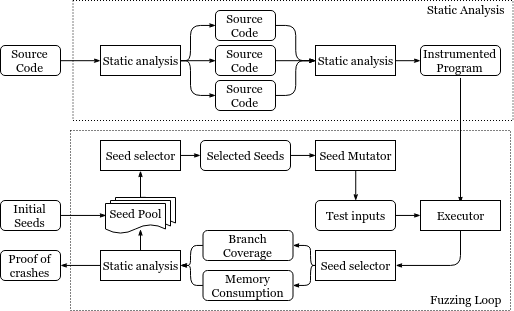
\includegraphics[width=\textwidth]{Chapter3/Memlock.png}
    \centering
    \caption{Memlock's approach} 
    \label{fig:memlock}
\end{figure}

